%% Für Bindekorrektur als optionales Argument "BCORfaktormitmaßeinheit", dann
% sieht auch Option "twoside" vernünftig aus
% Näheres zu "scrartcl" bzw. "scrreprt" und "scrbook" siehe KOMA-Skript Doku
\documentclass[12pt,a4paper,titlepage,headinclude,bibtotoc]{scrartcl}


%---- Allgemeine Layout Einstellungen ------------------------------------------

% Für Kopf und Fußzeilen, siehe auch KOMA-Skript Doku
\usepackage[komastyle]{scrpage2}
\pagestyle{scrheadings}
\setheadsepline{0.5pt}[\color{black}]

\usepackage{amsmath}

\usepackage{floatflt}

\setlength{\parindent}{0pt}

\usepackage{listings}

\usepackage{float}

%Einstellungen für Figuren- und Tabellenbeschriftungen
\setkomafont{captionlabel}{\sffamily\bfseries}
\setcapindent{0em}

%---- Weitere Pakete -----------------------------------------------------------
% Die Pakete sind alle in der TeX Live Distribution enthalten. Wichtige Adressen
% www.ctan.org, www.dante.de

% Sprachunterstützung
\usepackage[ngerman]{babel}

% Benutzung von Umlauten direkt im Text
% entweder "latin1" oder "utf8"
\usepackage[utf8x]{inputenc}
%\usepackage[utf8]{inputenc}

% Pakete mit Mathesymbolen und zur Beseitigung von Schwächen der Mathe-Umgebung
\usepackage{latexsym,exscale,stmaryrd,amssymb,amsmath}

% Weitere Symbole
\usepackage[nointegrals]{wasysym}
\usepackage{eurosym}

% Anderes Literaturverzeichnisformat
%\usepackage[square,sort&compress]{natbib}

% Für Farbe
\usepackage{color}

\usepackage{graphicx}

\usepackage[euler]{textgreek}

\usepackage{wrapfig}

\usepackage{subfigure}

\usepackage{sidecap}

% Befehl für "Entspricht"-Zeichen
\newcommand{\corresponds}{\ensuremath{\mathrel{\widehat{=}}}}

%Für chemische Formeln (von www.dante.de)
%% Anpassung an LaTeX(2e) von Bernd Raichle
\makeatletter
\DeclareRobustCommand{\chemical}[1]{%
  {\(\m@th
   \edef\resetfontdimens{\noexpand\)%
       \fontdimen16\textfont2=\the\fontdimen16\textfont2
       \fontdimen17\textfont2=\the\fontdimen17\textfont2\relax}%
   \fontdimen16\textfont2=2.7pt \fontdimen17\textfont2=2.7pt
   \mathrm{#1}%
   \resetfontdimens}}
\makeatother

\definecolor{source_green}{rgb}{0,0.6,0}
\definecolor{source_gray}{rgb}{0.5,0.5,0.5}
\definecolor{source_mauve}{rgb}{0.58,0,0.82}

\lstset{
  language=C++,                % choose the language of the code
  numbers=left,                   % where to put the line-numbers
  stepnumber=1,                   % the step between two line-numbers.        
  numbersep=5pt,				% how far the line-numbers are from the code
  basicstyle=\small,                  
  backgroundcolor=\color{white},  % choose the background color. You must add \usepackage{color}
  showspaces=false,               % show spaces adding particular underscores
  showstringspaces=false,         % underline spaces within strings
  showtabs=false,                 % show tabs within strings adding particular underscores
  tabsize=2,                      % sets default tabsize to 2 spaces
  captionpos=b,                   % sets the caption-position to bottom
  breaklines=true,                % sets automatic line breaking
  inputencoding=utf8,
   extendedchars=true,
   literate={á}{{\'a}}1 {ã}{{\~a}}1 {é}{{\'e}}1,
  keywordstyle=\color{blue},
  numberstyle=\tiny\color{source_gray},
  stringstyle=\color{source_mauve},
  commentstyle=\color{source_green},
  breakatwhitespace=true,         % sets if automatic breaks should only happen at whitespace
  title=\lstname,                 % show the filename of files included with \lstinputlisting;
}


\begin{document}

\begin{titlepage}
\centering
\textsc{\Large Numerische Strömungsmechanik\\
[1.5ex] Sommersemester 2016}

\vspace*{4.2cm}

\rule{\textwidth}{1pt}\\[0.5cm]
{\huge \bfseries
  Hausaufgabe\\[1.5ex]}
\rule{\textwidth}{1pt}

\vspace*{3.5cm}

\begin{Large}
\begin{tabular}{ll}
Name: & Roland Zimmermann\\
Matrikelnummer:	& 21426901 \\
Mail Adresse: & roland.zimmermann@stud.uni-goettingen.de \\ 
\\
Abgabetermin: & 05.08.2016\\
\end{tabular}
\end{Large}

\end{titlepage}



\tableofcontents

\newpage

\section{Einleitung}
\label{sec:einleitung}

\section{Fragestellung}
\label{sec:fragestellung}
In dieser Hausaufgabe wird ein zweidimensionales quadratisches System betrachtet. In diesem soll die Wärmeausbreitung (siehe \ref{sec:diff_adv}) beschrieben werden, welche durch ein extern erzeugtes Geschwindigkeitsfeld (durch einen Ventilator) hervorgerufen wird. Dieses Vektorfeld soll nicht zeitabhängig sein, und lässt sich in dimensionsloser Form durch
\begin{align*}
\vec{v} = (\pi \sin(2\pi x) \cos(\pi y), -2 \pi \cos(2\pi x) \sin(\pi y))^t
\end{align*}
beschreiben. Hierbei gibt es für jeden der vier Ränder je eine Randbedingung. So soll die Temperatur auf dem oberen Rand $T=1$ betragen, auf dem unteren dagegen $T=0$. An dem linken und rechten Rand soll dagegen bloß die jeweilige Normalenableitung verschwinden. Dies wird durch eine wärmeisoliernde Wand in dem System bedingt. Zu Beginn soll eine Temperaturverteilung der Form $T_{start} = y$ vorliegen.\\

Zur Untersuchung des System fallen mehrere Aufgaben an. So wird zuerst das Geschwindigkeitsfeld selber untersucht (siehe \ref{sec:task1}). Anschließend wird eine erste numerische Lösung des Problems (im \textit{FTCS-Schema}) durchgeführt (siehe \ref{sec:task2}). Daraufhin wird nun die numerische Korrektheit dieser Lösung untersucht (siehe \ref{sec:task3}). Schließlich werden für verschiedene Parameter Simulationen durchgeführt, um unter anderem die Stabilität zu beurteilen (siehe \ref{sec:task4}, \ref{sec:task5}). Schließlich wird das Problem noch einmal gelöst, diesmal aber im \textit{BTCS-Schema} (siehe \ref{sec:task6}).

\section{Theorie}
\label{sec:theorie}
\subsection{Die Diffusions-Advektion-Gleichung}
\label{sec:diff_adv}
Die Ausbreitung von Flüssigkeiten, Gasen beziehungsweise von Energie kann zum einen durch die \textit{Diffusionsgleichung}
\begin{align}
\label{eq:diff}
\frac{\partial}{\partial t}T = D \nabla^2 T 
%= D \left(\frac{\partial^2}{\partial x^2} + \frac{\partial^2}{\partial y^2} \right)T
\end{align}


und zum anderen durch die \textit{Advektionsgleichung}

\begin{align}
\label{eq:adv}
\frac{\partial}{\partial t}T = - \nabla \cdot (\vec{v}\cdot T)
\end{align}
beschrieben werden. Hierbei stehen $T$ für die Verteilung der Energie (Temperatur), $t$ für die Zeit und $D$ für die Diffusionskonstante.
Während die \textit{Diffusionsgleichung} die zeitliche Ausbreitung der Partikel beziehungsweise der Energie, bedingt durch zufällige Bewegungen, beschreibt, beschreibt die \textit{Advektionsgleichung} den Partikelfluss der durch ein Geschwindigkeitsfeld herbeigeführt wird.\\
Fasst man diese beiden Effekte zusammen, so erhält man die \textit{Diffusions-Advektion-Gleichung}
\begin{align}
\frac{\partial}{\partial t}T = D \nabla^2 T - \nabla \cdot (\vec{v}\cdot T)
%= D \left(\frac{\partial^2}{\partial x^2} + \frac{\partial^2}{\partial y^2} \right)T - (\frac{\partial}{\partial x} + \frac{\partial}{\partial y}) (\vec{v}\cdot T)
\end{align}
Hierbei kann nun, wenn ein gegebenen externes, divergenzfreies Geschwindigkeitsfeld gegeben ist, dieses aus der Divergenz herausgelöst werden, sodass sich
\begin{align}
\label{eq:orig_diff_adv}
\frac{\partial}{\partial t} T + \vec{v} \cdot \nabla T = D \nabla^2 T
\end{align}
ergibt.\\
Durch das Einführen der \textit{Péclet-Zahl}
\begin{align*}
Pe = \frac{L v \rho c_p}{\lambda}
\end{align*}
ist eine Entdimensionalisierung der Gleichung (\ref{eq:orig_diff_adv}) möglich. Hierbei stehen $L$ für eine charakteristische Länge, $v$ für eine Geschwindigkeit, $rho$ für die Dichte, $c_p$ für die spezifische Wärmekapazität und $\lambda$ für die Wärmeleitfähigkeit des jeweiligen Mediums. Somit ergibt sich
\begin{align}
\label{eq:diff_adv}
\frac{\partial}{\partial t} T + Pe \cdot \vec{v} \cdot \nabla T = \nabla^2 T
\end{align}

\subsection{Das FTCS-Schema}
Eine mögliche Methode zur Lösung einer solchen partiellen Differenzialgleichung ist durch die Verfahrensgruppe der finiten Differenzen gegeben. Eine hierfür geeignete Diskretiserung des Problems ist in Form eines \textit{FTCS}-Schemas (Forward in Time, Centered in Space) gegeben. Hierbei wird der Raum in der $x$-Richtung in $(N_x+1)$- und in der $y$-Richtung in $(N_y+1)$ Stützstellen unterteilt, sodass sich ein räumliches Gitter ergibt. Zwischen diesen Punkten herrscht ein jeweiliger Abstand von $\Delta x = X/N_x$ und $\Delta y = Y/N_y$, wobei $X$ und $Y$ für die Ausmaße des zu beschreibenden Problems in der $x$- und $y$-Richtung sind.\\
Die Temperatur $T(x, y)$, die hiermit beschrieben werden soll, geht somit in die Form $T_{i,j}$ über, wobei $i$ der Index des Punktes in der $x$- und $j$ der in der $y$-Richtung ist. Diese Indizes laufen von $0$ bis $N_x$ beziehungsweise $N_y$.\\
Um nun noch die Zeit zu erfassen, wird auch diese in Punkte diskretisiert, die einen Abstand $\Delta_t$ haben. Sodass sich insgesamt ein dreidimensionaler Würfel ergibt, dessen verschiedenen Ebenen für die verschiedenen Zeitpunkte stehen. Erneut geht die Temperatur $T(x, y) = T_{i,j}$ über in $T_{i,j}^N$, wobei $N$ für den zeitlichen Index steht. Auch hier wird von $0$ an indiziert.\\

Diese Aufteilung erlaubt es nun, die in den Gleichung (\ref{eq:diff_adv}) vorkommenden Ableitungen zu beschreiben.   
Hierbei wird in dem \textit{FTCS}-Schema die zeitliche Ableitung in der ersten und die räumlichen in der zweiten Ordnung beschrieben.
Es ergibt sich für die Ableitungen
\begin{align}
\frac{\partial}{\partial t}T(x,y) &= \frac{T_{i,j}^{N+1} - T_{i,j}^{N}}{\Delta t}, \\
\frac{\partial}{\partial x}T(x,y) &= \frac{T_{i+1,j}^{N} - T_{i-1,j}^{N}}{2 \Delta x}, \\
\frac{\partial^2}{\partial x^2}T(x,y) &= \frac{T_{i+1,j}^{N} - 2 T_{i,j}^{N} + T_{i-1,j}^{N}}{ \Delta x^2}.
\end{align}

Durch Einsetzen in die Gleichung (\ref{eq:diff_adv}) und Umstellen nach $T_{i,j}^{N+1}$ erhält man schließlich in der zweiten räumlichen Ordnung
\begin{align}
\label{eq:ftcs}
T_{i,j}^{N+1} = &T_{i,j}^N + \Delta t \left( -Pe \left( v^x_{i,j} \frac{T_{i+1,j}^N-T_{i-1,j}^N}{2\Delta x}+v^y_{i,j} \frac{T_{i,j+1}^N-T_{i,j-1}^N}{2\Delta x} \right) \right. \nonumber \\ 
 & \left.+ \frac{ T_{i+1,j}^N - 2 T_{i,j}^N +  T_{i-1,j}^N }{\Delta x^2} 
+ \frac{ T_{i,j+1}^N - 2  T_{i,j}^N + T_{i,j-1}^N}{\Delta y^2} \right) 
\end{align}
womit die Integration durchgeführt werden kann. Die Ausdrücke $v^x$ und $v^y$ stehen für die jeweilige $x$- und $y$-Komponente des zeitlich konstanten Geschwindigkeitsfeldes an dem jeweiligen Ort.\\
Des Weiteren sind allerdings noch die Randbedingungen zu beachten. Bei \textit{Dirichlet}-Rändern muss an dem Schema nichts geändert werden. Bei \textit{Neumann}-Rändern dagegen schon. Exemplarisch wird hierfür als Beispiels der linke Rand betrachtet, auf dem die erste Ableitung in $x$-Richtung verschwinden soll. Durch eine Taylor-Entwicklung und einen Koeffizientenvergleich erhält man die diskretisierte Randbedingung zweiter Ordnung
\begin{align*}
T_{i,j}^{N+1} - \frac{4}{3} T_{i+1,j}^{N+1} + \frac{1}{3} T_{i+2,j}^{N+1} = 0.
\end{align*}


\subsection{Das BTCS-Schema}
\label{sec:btcs}
Ein alternativer Ansatz zur Lösung ist das \textit{BTCS}-Schema (Backward in Time, Centered in Space), bei der räumlich erneut eine Diskretisierung zweiter Ordnung durchgeführt wird, diese allerdings zum Zeitpunkt $(N+1)$ ausgewertet wird. Zeitlich wird auch wieder ein Verfahren erster Ordnung verwendet.
Somit ergibt sich der Ausdruck
\begin{align}
\label{eq:impli}
T_{i,j}^{N} = T_{i,j}^{N+1} \alpha + \beta^-_{i-1,j} T_{i-1,j}^{N+1} + \beta^+_{i+1,j} T_{i+1,j}^{N+1} + \gamma^-_{i,j-1} T_{i,j-1}^{N+1} + \gamma^+_{i,j+1} T_{i,j+1}^{N+1}.
\end{align}
Dabei wurden die folgenden Abkürzungen eingeführt und benutzt
\begin{align}
\alpha &= \Delta t \left(\frac{1}{\Delta x^2} + \frac{1}{\Delta y^2} + \frac{1}{\Delta t} \right), \\
\beta^\pm_{i,j} &= \Delta t \left(-\frac{1}{\Delta x^2} \pm \frac{Pe v^x_{i,j}}{2 \Delta x}\right), \\
\gamma^\pm_{i,j} &= \Delta t \left(-\frac{1}{\Delta y^2} \pm \frac{Pe v^y_{i,j}}{2 \Delta y}\right).
\end{align}

Um das Problem nun besser beschreiben zu können, wird das zweidimensionale Feld in einen eindimensionalen Spaltenvektor zusammengefasst. Hierfür ist es notwendig, die Indizes umzubenennen. Hierbei wird ab jetzt die folgende Konvention benutzt: durchlaufe erst alle $x$-Werte zu einem festen $y$-Wert, und erhöhe das $y$. Dies bewirkt, dass die Zeilen des Feldes hintereinander geschrieben werden:
\begin{align*}
T_{i,j}^{N} = T_{i+N_y j}^{N}.
\end{align*}
Nun kann die Gleichung (\ref{eq:impli}) als eine Matrixoperation der Form
\begin{align*}
\vec{T}^N = M \cdot \vec{T}^{N+1},
\end{align*} 
mit der Matrix $M$ ausgedrückt werden.
Diese hat die fünf Diagonalen, die ungleich null sind in ihrem Hauptteil, und zwei weitere Submatrizen, die fast nur eine Hauptdiagonale haben, die ungleich null ist.
Somit schreibe $M$ nun als Blockmatrix
\begin{align*}
 \boldsymbol{M}  =  \begin{pmatrix}
  A  & 0 & 0 \\
  0  & B & 0 \\
  0  & 0 & C \\
 \end{pmatrix}
 ,
\end{align*}
mit der Matrix $A$ 
\begin{align*}
\boldsymbol{A} =
  \begin{pmatrix}
  2  & -4/3 & 1/3 & . & 1/3 & -4/3 & 2 & -4/3 & 1/3 & .\\
  0  & 1 & 0 & . &   &   &   &   &   & . \\
  0  & 0 & 1 & 0 & . &   &   &   &   & . \\
  .  & . & . & . & . & . &   &   &   & . \\
  .  &   & . & . & . & . & . &   &   & . \\
  .  &   &   & . & . & . & . & . & . & . \\
  .  &   &   &   & . & . & . & . & . & . \\
  .  &   &   &   &   & . & . & . & . & . \\
  .  &   &   &   &   &   & . & 0 & 1 & 0 \\
  0  & . & . & . & . & . & . & . & 0 & 1 \\
 \end{pmatrix}
 ,
 \end{align*}
 welche die Randbedingungen am oberen, linken und rechten Rand umsetzt; und der Matrix $C$

 \begin{align*}
 \boldsymbol{C}  =
  \begin{pmatrix}
  1  & 0 & . & . & 0 \\
  0  & 1 & 0 & . & . \\
  .  & . & . & . & . \\
  .  &   & 0 & 1 & 0 \\
  0  & . & . & 0 & 1 \\
  \end{pmatrix}
  ,
\end{align*}
\setcounter{MaxMatrixCols}{25}
welche die Randbedingungen am unteren Rand umsetzt. Die Matrix $B$
\begin{align*}
\boldsymbol{B} =
  \begin{pmatrix}
  \gamma^-  & . & \beta^- & \alpha & \beta^+ & . & \gamma^+ & 0 & .& .& 0 \\
  0  & \gamma^- & . & \beta^- & \alpha  & \beta^+  & .  & \gamma^+  & 0 &  .& 0 \\
  0  & 0 & \gamma^- & . & \beta^- & \alpha & \beta^+ & .  & \gamma^+  & .& 0 \\
  .  &   & . & . & . & . & .  & .  & .  & .  & . \\
  .  &   &   & . & . & . & . & .  & .  & .  & . \\
  .  &   &   &   & . & . & . & . & . & .  & . \\
  .  &   &   &   &   & . & . & . & . & . & .  \\
  .  &   &   &   &   &   & . & . & . & .  & . \\
  .  &   &   &   &   &   &   & . & . & .  & . \\
  0  & . & 0 & \gamma^- & . & \beta^- & \alpha & \beta^+ & .  & \gamma^+  & . \\
  0  & . & . & 0 & \gamma^- & . & \beta^- & \alpha & \beta^+ & .  & \gamma^+  \\
 \end{pmatrix}
 ,
 \end{align*}
setzt die implizite Gleichung (\ref{eq:impli}) um. Um nun einen Zeitschritt vorzugehen, muss also nur noch die Matrix $M$ invertiert werden, beziehungsweise das Gleichungssystem $M \vec{x} = \vec{b}$ gelöst werden.\\
Hierfür hat sich das \textit{SOR-Verfahren}, welches eine Modifikation des \textit{Gauß-Seidel-Verfahrens} ist, als besonders geeignet herausgestellt. Dies sind beides iterative Lösungsverfahren. Um diese zu benutzen, wird die Matrix zuerst in drei Teilmatrizen $\boldsymbol{M}=\boldsymbol{L}+\boldsymbol{D}+\boldsymbol{U}$ zerlegt, wobei $D$ eine Diagonal-, $L$ eine untere Dreiecks- und $U$ eine obere Dreiecksmatrix ist. Zudem wird der \textit{Residuen-Vektor} $\vec{r_n} = \boldsymbol{M} \vec{x_n} - \vec{b}$ eingeführt, wobei der Index den jeweiligen Iterationsschritt angibt. Dieser Vektor beschreibt die Differenz zwischen der korrekten und der iterativen Lösung der Gleichung $M x = b$.\\
Durch diese Zerlegung ist es möglich eine rekursive Bestimmungsformel [2, S. 25ff]
\begin{align*}
\vec{x}^{\,n} = \vec{x}^{\,n-1} - \alpha(\boldsymbol{L}+\boldsymbol{D})^{-1} \vec{r}^{\,n-1}
\end{align*}
aufzustellen. Hierbei ist $\alpha$ der so genannte \textit{Relaxationsparameter}. Bei dem \textit{Gauss-Seidel-Verfahren} ist er gleich null.\\
Diese Matrizen-Gleichung kann in Summenschreibweise durch Eigenschaften triagonaler Matrizen aus der linearen Algebra auch als
\begin{align}
\label{eq:sor}
x^{n+1}_i = (1-\alpha)x^{n}_i + \frac{\alpha}{m_{i,i}} \left(b_i - \sum\limits_{j=1}^{i-1} m_{i,j} x^{n+1}_j - \sum\limits_{j=i}^{N} m_{i,j} x^{n}_j \right)  
\end{align}
aufgefasst werden [2, S.30], wobei $N$ die Dimensionen des Problems angibt.

\section{Durchführung der Aufgaben}
\subsection{Aufgabe 1: Untersuchung von $\vec{v}$}
\label{sec:task1}
Für die numerische Betrachtung des Problems spielt der Einfluss von $\vec{v}$ eine entscheidende Rolle. Ist dieses Geschwindigkeitsfeld nämlich divergenzfrei, so ergibt sich eine mögliche, vereinfachende Betrachtung in diskretisierter Form (siehe ). Für das externe Feld
\begin{align*}
\vec{v} = (\pi \sin(2\pi x) \cos(\pi y), -2 \pi \cos(2\pi x) \sin(\pi y))^t
\end{align*}
gilt
\begin{align*}
\nabla \cdot \vec{v} = \frac{\partial}{\partial x} (\pi \sin(2\pi x) \cos(\pi y) + \frac{\partial}{\partial y} (-2 \pi \cos(2\pi x) \sin(\pi y)) = 0;
\end{align*}
es ist somit divergenzfrei. Dies kann man auch grafisch nachvollziehen.
\begin{figure}[H]
 \centering
   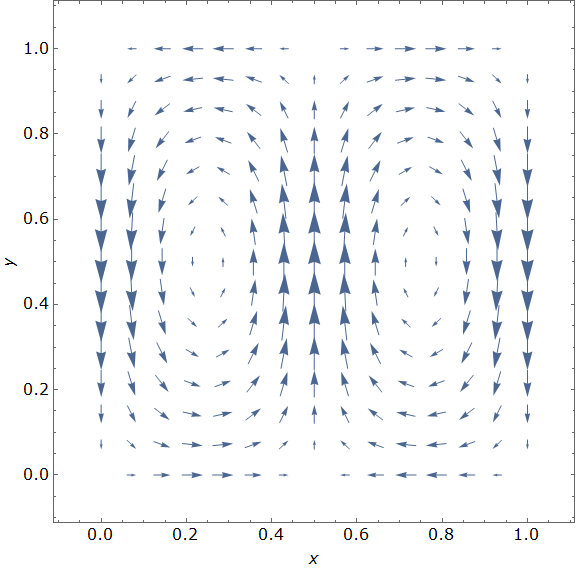
\includegraphics[width=0.6\textwidth]{res/task1.png}
   \caption{Grafische Darstellung des Geschwindigkeitsfeldes $\vec{v}$ in Abhängigkeit von $x$ und $y$.}
 \label{fig:aufbaue_bild}
\end{figure}

\subsection{Aufgabe 2: FTCS-Lösung}
\label{sec:task2}

\subsection{Aufgabe 3: Numerische Korrektheit der FTCS-Lösung}
\label{sec:task3}
Zur Beurteilung der Korrektheit der numerischen Lösung wird normalerweise erstmal versucht, das Ergebnis mit der analytischen Lösung zu vergleichen. Da dieses Problem allerdings nicht analytisch lösbar ist, muss hier anders verfahren werden. Als Ansatz hierbei wird eine mögliche stationäre Lösung geraten, und die Differenzialgleichung um einen Quellterm so ergänzt, dass dies die exakte Lösung des Problems ist.\\
Für diese konstruierte stationäre Lösung wird der Ansatz
\begin{align*}
T^* = \cos(\pi x) \sin(\pi y) + y
\end{align*} 
gewählt, da dies sowohl die Startverteilung umsetzt, als auch die vier Randbedingungen erfüllt.
Um den Quellterm $Q$ zu korrigieren, wird $T^*$ in die stationäre Gleichung
\begin{align*}
Pe \cdot \vec{v} \nabla T^* = \nabla^2 T^* + Q 
\end{align*}
eingesetzt, welche auch Quellen berücksichtigt. Es ergibt sich somit
\begin{align*}
Q = Pe \cdot \vec{v} \nabla T^* - \nabla^2 T^*,
\end{align*}
was sich nach Einsetzen des Ansatzes und des gegebenen Geschwindigkeitsfeldes zu
\begin{align*}
Q = \pi^2 \left(2 \cos(\pi x) \sin(\pi y) - Pe \cdot \cos(\pi x)^3 \sin(2 \pi y) \right) - 2 Pe \cdot \pi \cos(2 \pi x) \sin(\pi y)
\end{align*}
ergibt.\\
Berücksichtigt man diesen Quellterm in dem \textit{FTCS-Schema}, folgt:
\begin{align*}
T_{i,j}^{N+1} = &T_{i,j}^N + \Delta t \left( -Pe \left( v^x_{i,j} \frac{T_{i+1,j}^N-T_{i-1,j}^N}{2\Delta x}+v^y_{i,j} \frac{T_{i,j+1}^N-T_{i,j-1}^N}{2\Delta x} \right) \right. \nonumber \\ 
 & \left.+ \frac{ T_{i+1,j}^N - 2 T_{i,j}^N +  T_{i-1,j}^N }{\Delta x^2} 
+ \frac{ T_{i,j+1}^N - 2  T_{i,j}^N + T_{i,j-1}^N}{\Delta y^2} + Q_{i,j} \right) 
\end{align*}

Dies führt zu Änderungen des Quellcodes im Vergleich zur vorherige Aufgabe in der Methode ... in den Zeilen ...-... .
Nun kann zu jedem Zeitpunkt die Differenz zwischen der stationären Lösung $T_{i,j}^*$ und der numerischen Lösung $T_{i,j}^N$ berechnet werden als
\begin{align*}
\sigma^N = \sqrt(\Sigma_{i,j} (T_{i,j}^N - T_{i,j}^*)^2 ).
\end{align*}
Diese Abweichung wird nun alle $100$ Zeitschritte ausgegeben. Dies führt zu Veränderungen in der Methode ... in Zeile ... bis ... .\\
Setzt man nun noch $N_x = N_y$, und variiert diese Werte für ein festes $\Delta t$, so können Aussagen getroffen werden, über die Abweichungen der stationären numerischen $T$ und der tatsächlichen stationären Lösung $T^*$ in Abhängigkeit von der Gittergröße.

\begin{figure}[H]
 \centering
   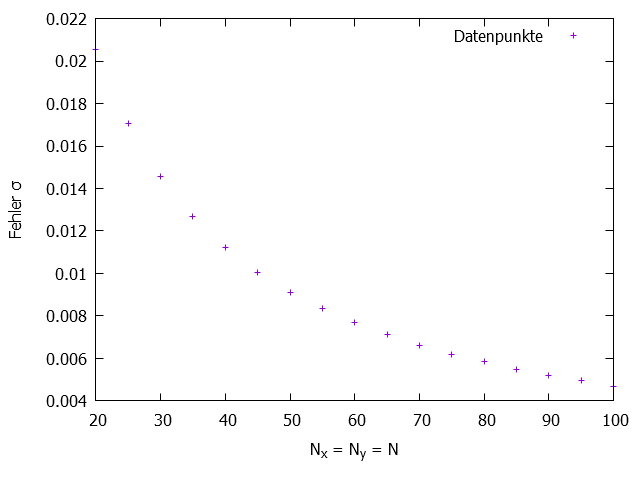
\includegraphics[width=0.7\textwidth]{res/task3.png}
   \caption{Grafische Auftragung der numerischen Abweichung $\sigma$ in Abhängigkeit von der Gittergröße $N$.}
 \label{fig:task3}
\end{figure}

In Abbildung (\ref{fig:task3}) ist der Verlauf des Fehlers $\sigma$ in Abhängigkeit von $N_x = N_y$ für $Pe = 2$ für einen Zeitschritt von $\Delta t = 2 \cdot 10^{-5}$ aufgetragen.
Zudem wurde eine eine Regression durchgeführt, welche eine Abhängigkeit der Form $\sigma = N^{-1.2}$ ergeben hat. Dazu ist noch anzumerken, dass für größere $N$-Werte (größer als $115$) der Fehler nicht mehr weiter sinkt, sondern sogar stark anwächst, da die numerische Lösung divergent wird.


\subsection{Aufgabe 4: Auswertung verschiedener FTCS-Lösungen}
\label{sec:task4}
Im weiteren Verlauf wird der zuvor eingeführte Quellterm $Q=0$ gesetzt. Nun kann das Temperaturfeld $T$ für zwei verschiedene \textit{Péclet-Zahlen} $Pe = 2$ und $Pe = 10$ simuliert, und zu den drei Zeitpunkten $t = 0.005$, $t = 0.05$ und $t=0.5$ visualisiert werden. Hierfür wird $\Delta t = 2 \cdot 10^-4$ und $N=N_x=N_y = 30$ angenommen. Die Darstellungen sind in den Abbildungen (\ref{fig:task4_2}) und (\ref{fig:task4_10}) zu finden.

\noindent\begin{minipage}[t]{0.50\textwidth}% adapt widths of minipages to your needs
\begin{figure}[H]  
   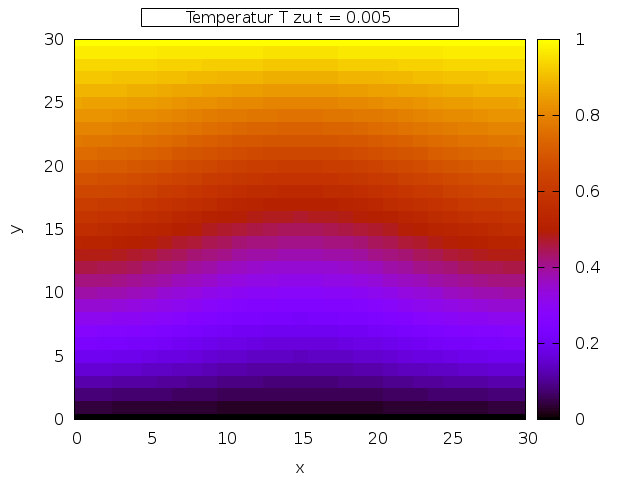
\includegraphics[width=\linewidth]{res/task4/2_0005.png}
   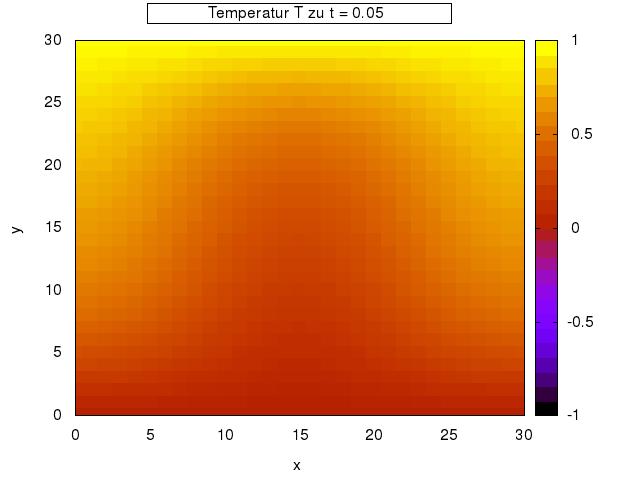
\includegraphics[width=\linewidth]{res/task4/2_005.png}
   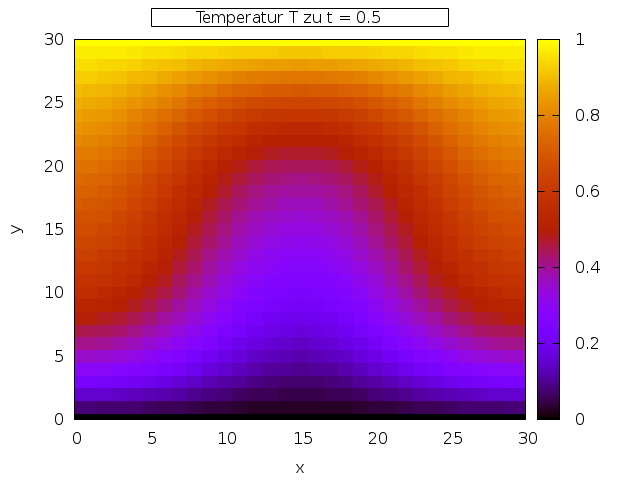
\includegraphics[width=\linewidth]{res/task4/2_05.png}
   \caption{Temperatur für $Pe = 2$.}
   \label{fig:task4_2}
   \end{figure}
\end{minipage}%
\hfill%
\noindent\begin{minipage}[t]{0.50\textwidth}% adapt widths of minipages to your needs
\begin{figure}[H]  
   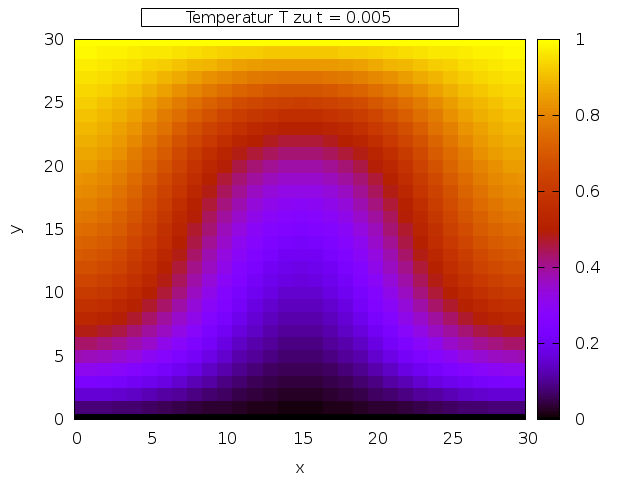
\includegraphics[width=\linewidth]{res/task4/10_0005.png}
   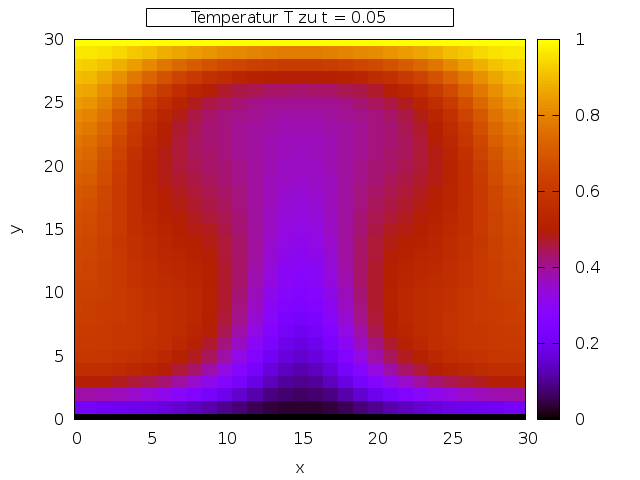
\includegraphics[width=\linewidth]{res/task4/10_005.png}
   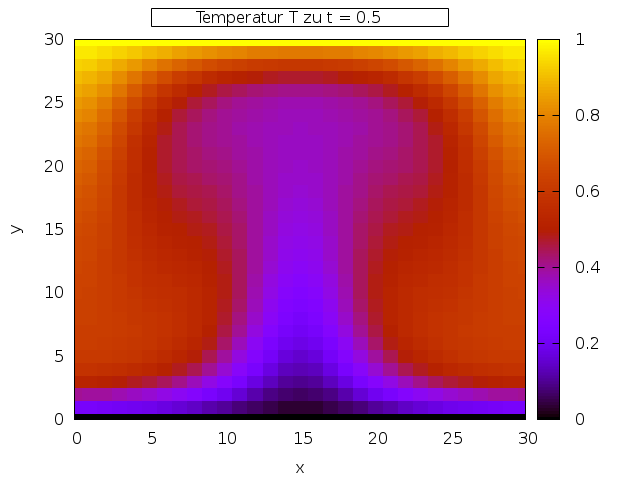
\includegraphics[width=\linewidth]{res/task4/10_05.png}
   \caption{Temperatur für $Pe = 10$.}
   \label{fig:task4_10}
   \end{figure}
\end{minipage}%
\hfill%


\subsection{Aufgabe 5: Beurteilung der Stabilität der FTCS-Lösung}
\label{sec:task5}
Um weitere Aussagen über die numerische Lösung treffen zu können, wird nun noch die Stabilität betrachtet. Hierfür wird zuerst für $N=N_x=N_y = 30$ die maximale Zeitschrittgröße $\Delta t^{Pe}_{max}$ für die \textit{Péclet-Zahlen} $Pe \in \{0.1, 1.0, 10\}$ bestimmt.\\
Diese ergeben sich zu
\begin{align*}
\Delta t^{0.1}_{max} &= 2.785 \cdot 10^{-4} 2.788, \\
\Delta t^{1.0}_{max} &= 2.787 \cdot 10^{-4} 2.789, \\
\Delta t^{10}_{max}  &= 2.795 \cdot 10^{-4} .
\end{align*}
Dies liefert einen ersten Eindruck: Die Stabilitätsgrenze hängt von $Pe$ ab, und nimmt für steigende $Pe$ in gewissen, geringen Maßen zu.\\
Für eine genauere Aussage wird nun eine \textit{von-Neumann-Stabilitätsanalyse} durchgeführt. Hierfür wird für die Lösung ein Ansatz der generellen Form
\begin{align*}
T^N_{i,j} = \xi^N e^{i(k_x \Delta x \cdot i + k_y \Delta y \cdot j)}
\end{align*}
gewählt.
Durch Einsetzen in Gleichung (\ref{eq:ftcs}) und Kürzen ergibt sich der Ausdruck
\begin{align*}
\xi = 1 - \frac{\Delta t Pe v^x}{2 \Delta x} \left( e^{i k_x \Delta x} - e^{-i k_x \Delta x} \right) - \frac{\Delta t Pe v^y}{2 \Delta y} \left( e^{i k_y \Delta y} - e^{-i k_y \Delta y} \right) -\frac{2 \Delta t}{\Delta x^2} - \frac{2 \Delta t}{\Delta y^2} \\
 + \frac{\Delta t}{\Delta x^2} \left( e^{i k_x \Delta x} + e^{-i k_x \Delta x} \right) +\frac{\Delta t}{\Delta y^2} \left( e^{i k_y \Delta y} + e^{-i k_y \Delta y} \right),
\end{align*}
welcher durch trigonometrische Identitäten in
\begin{align*}
\xi = 1 - i \Delta t Pe\left(\frac{ v^x }{\Delta x} \sin(k_x \Delta x) + \frac{v^y}{\Delta y}  \sin(k_y \Delta y) \right) + \frac{2 \Delta t}{\Delta x^2}\cos(k_x \Delta x) + \frac{2 \Delta t}{\Delta y^2}\cos(k_y \Delta y) \\-\frac{2 \Delta t}{\Delta x^2} - \frac{2 \Delta t}{\Delta y^2}
\end{align*}
übergeht. Damit das Verfahren konvergiert, muss $\xi$ kleiner $1$ ein. Nähert man hier den Sinus und den Cosinus mit den Maximalwerten, und schätzt die Komponenten $v^x$ und $v^y$ nach oben durch $\pi$ und $2\pi$ ab, so ergibt sich
\begin{align}
\lambda^2 \left(64 + \frac{Pe 2 \pi^2}{\Delta x^2} \right) -16 \lambda <0,
\end{align}
mit der \textit{CFL-Zahl} $\lambda = \Delta t/\Delta x^2$.
Eine Lösung dieser Ungleichung ergibt folgenden Bereich, sodass das \textit{FTCS-Schema} konvergiert:
\begin{align}
0 < \lambda = \frac{\Delta t}{\Delta x^2} < \frac{8 \left(\frac{Pe}{\Delta x}\right)^2}{32\left(\frac{Pe}{\Delta x}\right)^2 + \pi^2}.
\end{align}
Dies ist durch die Abschätzungen nach oben bedingt, eine obere Schranke. Liegt $\lambda$ außerhalb des Bereiches, aber nahe an der Grenze, so ist ein Konvergieren nicht sicher ausgeschlossen. Liegt $\lambda$ allerdings in dem Bereich, so konvergiert das Verfahren sicher. Dieses Verhalten konnte an den zuvor empirisch ermittelten Grenzen für $\Delta t$ verifiziert werden.

\subsection{Aufgabe 6: BTCS-Lösung}
\label{sec:task6}
Nachdem zuvor die explizite Diskretisierung untersucht wurde, wird das Problem nun implizit im \textit{BTCS-Schema} betrachtet (siehe \ref{sec:btcs}). Hierfür wird zuerst die zuvor beschriebene Matrix $\textbf{M}$ implementiert. Dies wird in (...) durchgeführt. Nun muss nur noch in jedem Integrationsschritt diese Matrix invertiert werden. Dafür wurde das \textit{SOR-Verfahren} in (...) nach Gleichung (\ref{eq:sor}) implementiert. Dabei werden in jedem einzelnen Interationsschritt die Residuen $\vec{r} = \textbf{M} \vec{x}-\vec{b}$ für die Lösung von $\textbf{M} \vec{x} = \vec{b}$ berechnet, und gefordert, dass der Betrag dieser kleiner als $|\vec{r}| < 10^{-4}$ ist. Dies wird als Abbruchbedingung im dem \textit{SOR-Verfahren} genutzt. Um die Vorteile des \textit{SOR} wirklich nutzen zu können, muss zuerst ein geeigneter Relaxationsparameter $\alpha$ ermittelt werden. Hierzu wird $Pe=10$, $N_x=N_y = 30$ und $\Delta t=100$ gesetzt. Nun wird $\alpha$ mit einer Schrittweite von $0.05$ ab $1.0$ variiert und die benötigten Iterationen ermittelt. 
\begin{figure}[H]
 \centering
   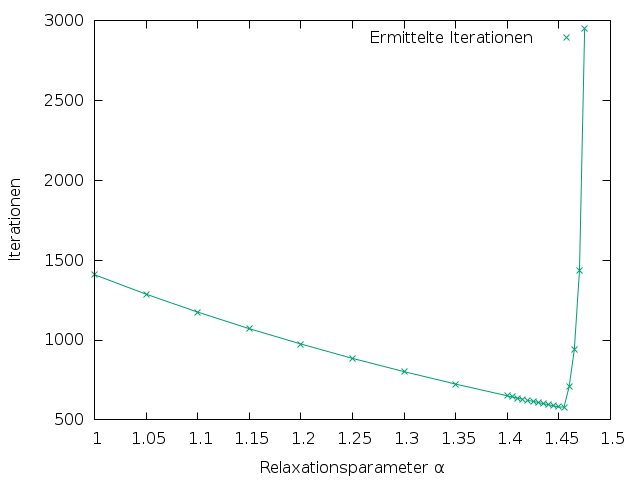
\includegraphics[width=0.65\textwidth]{res/task6/sor_parameter.png}
   \caption{Grafische Darstellung der benötigten Iterationen zur Konvergenz in Abhängigkeit vom Relaxationsparameter $\alpha$.}
 \label{fig:task6_param_comp}
\end{figure}
Die grafische Auftragung der so ermittelten Ergebnisse ist in Abbildung (\ref{fig:task6_param_comp}) zu finden. Es ist gut erkennbar, dass das bei $\alpha=1.41$ die geringste Anzahl an Iterationen benötigt wurde. Somit wird im weiteren Verlauf dieser Parameter genutzt.

\noindent\begin{minipage}[t]{0.55\textwidth}% adapt widths of minipages to your needs
\begin{figure}[H]  
   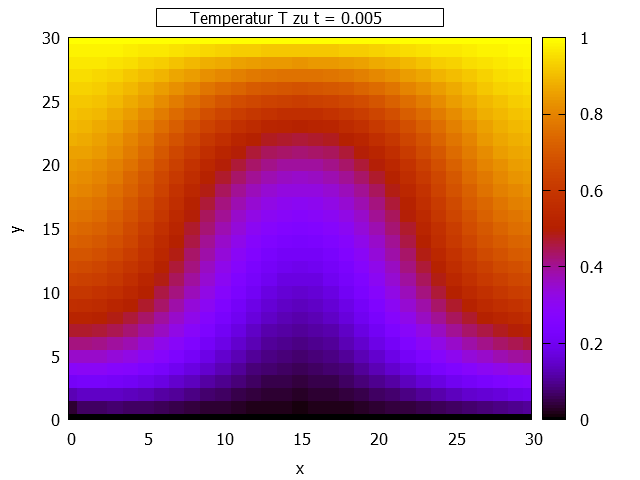
\includegraphics[width=\linewidth]{res/task6/grid0005.png}
   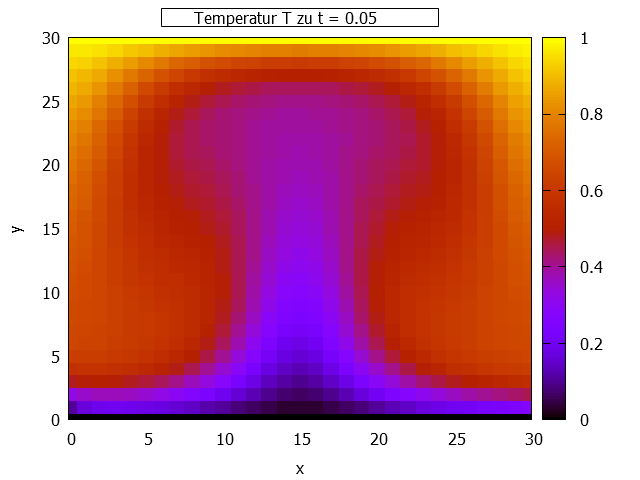
\includegraphics[width=\linewidth]{res/task6/grid005.png}
   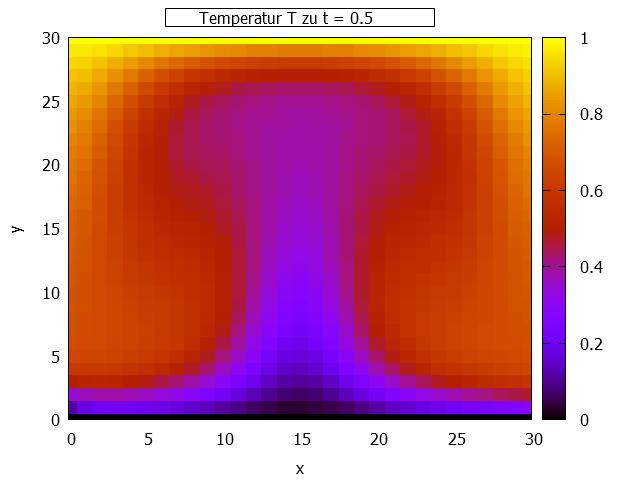
\includegraphics[width=\linewidth]{res/task6/grid05.png}
   \caption{Temperatur nach dem \textit{BTCS-Schema} für $Pe=10$ und $\Delta t = 2\cdot10^{-4}$.}
   \label{fig:task6}
   \end{figure}
\end{minipage}%
\hfill%
\noindent\begin{minipage}[t]{0.45\textwidth}% adapt widths of minipages to your needs
\vspace{1cm}
Schließlich wird das zuvor implementierte und getestete Verfahren noch einmal für die Parameterwahl aus Aufgabenpunkt (\ref{sec:task4}) angewendet, um die Ergebnisse miteinander zu vergleichen. Hierfür wurde also erneut $Pe = 10$, $\Delta t = 2 \cdot 10^{-4}$ und $t \in \{0.005, 0.05, 0.5\}$ gewählt. Die hierdurch erhaltenen Temperaturverteilungen sind erneut als Heatmap in Abbildung (\ref{fig:task6}) dargestellt.
\end{minipage}%
\hfill%

\section{Auswertung der Ergebnisse}
\label{sec:interpretation}
\subsection{Numerische Korrektheit der FTCS-Lösung}
\label{sec:disc_num_corr}
Durch den Vergleich in Abschnitt (\ref{sec:task3}) ist erkennbar, dass der numerische Fehler für größere Gitter deutlich geringer wird. Dieser Abfall hat allerdings auch eine bestimmte Grenze. Überschreitet $N = N_x = N_y$ diesen Wert, so kann die numerische Lösung nicht mehr konvergieren. Den Grund für dieses Verhalten (Abweichung der \textit{CFL-Zahl}) ist in Abschnitt (\ref{sec:task5}) beschrieben und erklärt. Anzumerken ist noch, dass der Fehler noch rapider gefallen wäre, wenn man den Gesamtfehler durch die Anzahl der zu berechnenden Gitterpunkte zwecks einer Normalisierung geteilt hätte.

\begin{thebibliography}{9}
  \bibitem{manmana}
  Andres Honecker, Thomas Pruschke, Salvatore R. Manmana, \\
  \emph{Scriptum zur Vorlesung: Computergestütztes wissenschaftliches Rechnen}. \\
 Göttingen,
  Sommersemester 2016

  \bibitem{sor}
  W. Auzinger, \\
  \emph{Lecture Notes Iterative Solution of Large Linear Systems}. \\
 Wien, 2011
 
 
 
 \end{thebibliography}
\clearpage

\appendix
\section{Quellcode}
\label{sec:source} 
\lstinputlisting{source/task02.cpp}
\lstinputlisting{source/task03.cpp}
\lstinputlisting{source/task06.cpp}

\end{document}